\chapter{力制御と位置制御の統合}
本章では,力制御と位置制御を統合させて油圧シリンダの制御を行う.
制御で実現させる動作の例を\figname\ref{fig5:forceandpositionIMAGE}に示す.
\figname\ref{fig5:forceandpositionIMAGE}は位置目標として正弦波目標を与えており,対象物(固定板)に触れていない時は位置目標に従い,対象物に触れたら力制御を行う例を示している.

\begin{figure}[b]
    \centering
        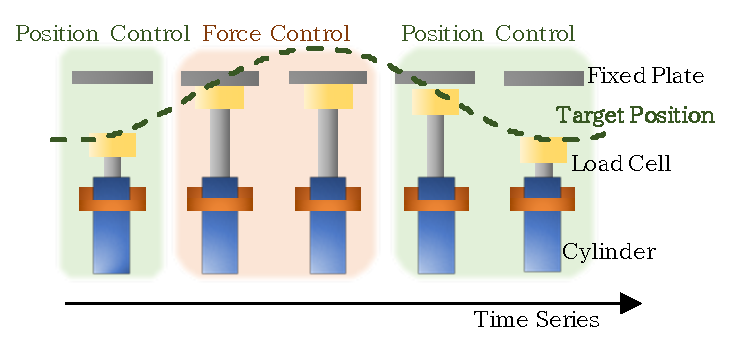
\includegraphics[keepaspectratio, scale=.9]{contents/IntegrationControl/figure/forceandpositionIMAGE.pdf}
        \caption{Image of Integration Control of Foce and Position}
        \label{fig5:forceandpositionIMAGE}
\end{figure}

制御にあたっては,(ⅰ)対象物に触れている時には力制御,それ以外には位置制御を行うというように力制御と位置制御を切り替える並列型の手法,(ⅱ)位置制御のからの入力をトルク入力と捉え,そのトルクを満たすように力制御を行う直列型の手法が考えられる.
また,直列型の手法を用いるとコンプライアンス制御を行うことも可能である.
そこで本章では並列型と直列型それぞれについて述べる.

\section{並列型制御手法}
並列型の手法の概略を\figname\ref{fig5:pararell_torqueandposition}に示す.
位置制御はPD制御で行い,Pゲインを15,Dゲインを0.1とした.
また,力制御はPID制御,I-PD制御,サーボ系$H_\infty$制御により行い,PID制御とI-PD制御のゲインはPゲイン8.4,Iゲイン168,Dゲイン0.1とし,サーボ系$H_\infty$の制御器にはむだ時間を無視して設計したコントローラ$K_{H_\infty\mathrm{servo}}$を用いる.
力制御と位置制御の切り替えは,以下のアルゴリズムにより行う.
\begin{itembox}[l]{切り替えアルゴリズム}
    \begin{enumerate}
        \item ロッド先端が対象物に触れていない場合は位置制御を行う.
        \item 対象物に触れており,かつ力目標による力の付加方向と位置目標による進行方向が``一致している''場合は力制御を行う.
        \item 対象物に触れており,かつ力目標による力の付加方向と位置目標による進行方向が``逆''の場合は位置制御を行う.
    \end{enumerate}
\end{itembox}

また,接触非接触の判定は\figname\ref{fig5:touch_define}に示すように,目標値に対する割合で判定を行う.
非接触から接触と接触から非接触の閾値が異なるのは,チャタリングを防ぐためである.
また,制御モードが切り替わった際には積分器のリセットを行っている.

\begin{figure}[t]
    \centering
        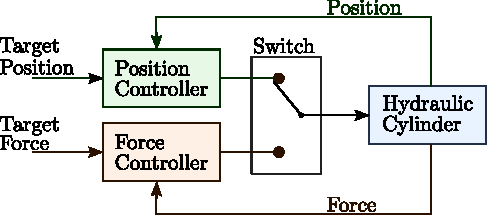
\includegraphics[keepaspectratio, scale=1.0]{contents/IntegrationControl/figure/pararell_torqueandposition.pdf}
        \caption{Force and Position Controller (Pararell)}
        \label{fig5:pararell_torqueandposition}
\end{figure}

\begin{figure}[t]
    \centering
        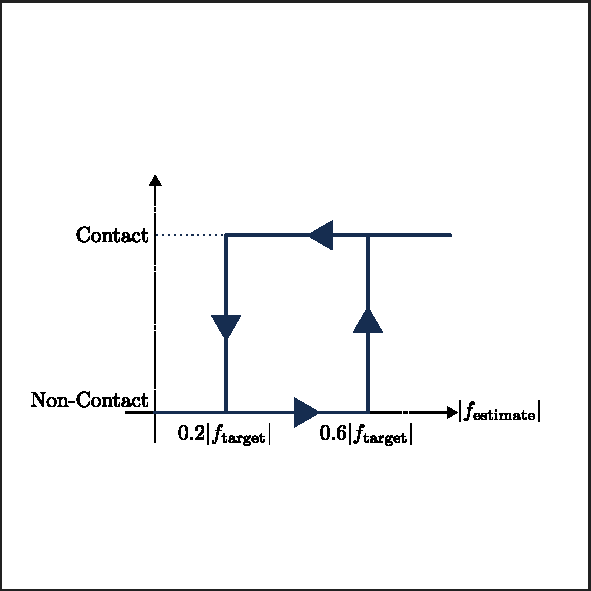
\includegraphics[keepaspectratio, scale=1.0]{contents/IntegrationControl/figure/touch_define.pdf}
        \caption{Decision of Touch or No Touch}
        \label{fig5:touch_define}
\end{figure}

力目標値として\SI{1}{kN},位置目標として振幅\SI{20}{mm},角振動数\SI{1}{rad/s}の正弦波を与える.
応答のようすを
\begin{figure}[t]
    \begin{minipage}{\minipageratio\hsize}
    \centering
        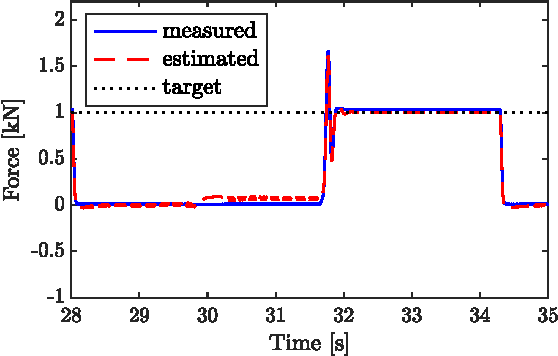
\includegraphics[keepaspectratio, scale = \minifigscale]{contents/IntegrationControl/figure/SECASQ/crop-FBsw_PID_force.pdf}
        \subcaption{$\fmsr$ and $\fest$}
        \label{fig5:crop-FBsw_PID_force}
    \end{minipage}
    \begin{minipage}{\minipageratio\hsize}
    \centering
        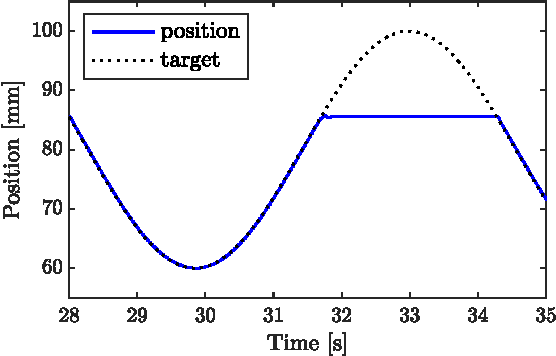
\includegraphics[keepaspectratio, scale = \minifigscale]
        {contents/IntegrationControl/figure/SECASQ/crop-FBsw_PID_pos.pdf}
        \subcaption{Position}
        \label{fig5:crop-FBsw_PID_pos}
    \end{minipage}
    \caption{Pararell Control (Position Controller:PD, Force Controller:PID)}   
    \label{fig5:crop-FBsw_PID}
\end{figure}

\begin{figure}[t]
    \begin{minipage}{\minipageratio\hsize}
    \centering
        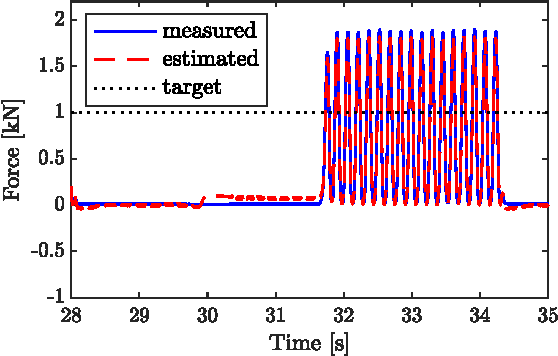
\includegraphics[keepaspectratio, scale = \minifigscale]{contents/IntegrationControl/figure/SECASQ/crop-FBsw_IPD_force.pdf}
        \subcaption{$\fmsr$ and $\fest$}
        \label{fig5:crop-FBsw_IPD_force}
    \end{minipage}
    \begin{minipage}{\minipageratio\hsize}
    \centering
        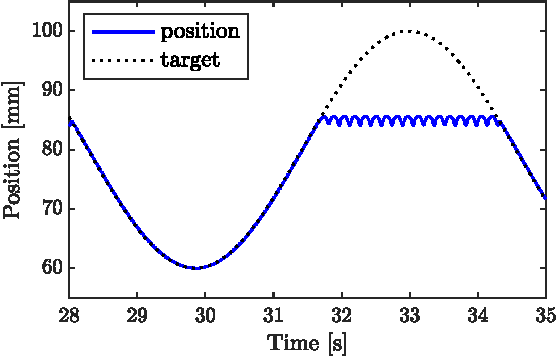
\includegraphics[keepaspectratio, scale = \minifigscale]
        {contents/IntegrationControl/figure/SECASQ/crop-FBsw_IPD_pos.pdf}
        \subcaption{Position}
        \label{fig5:crop-FBsw_IPD_pos}
    \end{minipage}
    \caption{Pararell Control (Position Controller:PD, Force Controller:I-PD)}
    \label{fig5:crop-FBsw_IPD}
\end{figure}

\begin{figure}[t]
    \begin{minipage}{\minipageratio\hsize}
    \centering
        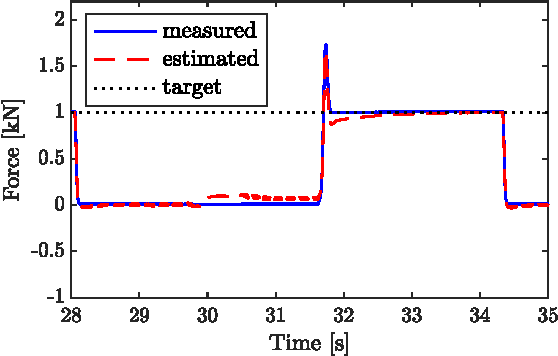
\includegraphics[keepaspectratio, scale = \minifigscale]{contents/IntegrationControl/figure/SECASQ/crop-FBsw_JFPS4_force.pdf}
        \subcaption{$\fmsr$ and $\fest$}
        \label{fig5:crop-FBsw_JFPS4_force}
    \end{minipage}
    \begin{minipage}{\minipageratio\hsize}
    \centering
        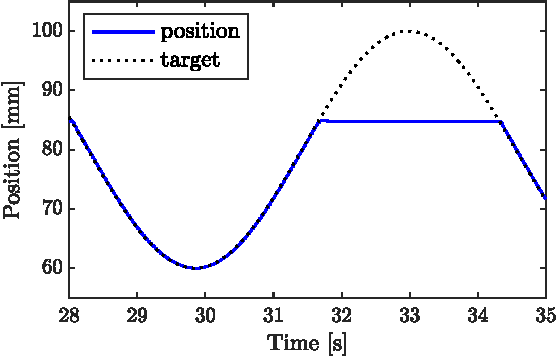
\includegraphics[keepaspectratio, scale = \minifigscale]
        {contents/IntegrationControl/figure/SECASQ/crop-FBsw_JFPS4_pos.pdf}
        \subcaption{Position}
        \label{fig5:crop-FBsw_JFPS4_pos}
    \end{minipage}
    \caption{Pararell Control (Position Controller:PD, Force Controller:$K_{H_\infty\mathrm{servo}}$)}   
    \label{fig5:crop-FBsw_JFPS4}
\end{figure}
% \begin{figure}[t]
%     \begin{minipage}{\minipageratio\hsize}
%     \centering
%         \includegraphics[keepaspectratio, width = \minifigwidth]
%         \subcaption{}
%         \label{fig5:}
%     \end{minipage}
%     \begin{minipage}{\minipageratio\hsize}
%     \centering
%         \includegraphics[keepaspectratio, width = \minifigwidth]
%         \subcaption{}
%         \label{fig5:}
%     \end{minipage}
%     \caption{}   
%     \label{fig5:}
% \end{figure}

\section{直列型制御手法}
\subsection{トルク補償による直列型制御}

% \begin{figure}[t]
%     \begin{minipage}{\minipageratio\hsize}
%     \centering
%         \includegraphics[keepaspectratio, scale = 1.0]{contents/IntegrationControl/figure/SECASQ/crop-FBcasq_PID_bothreset_force.pdf}
%         \subcaption{Force$\fmsr$ and Estimated Force $\fest$}
%         \label{fig5:crop-FBcasq_PID_bothreset_force}
%     \end{minipage}
%     \begin{minipage}{\minipageratio\hsize}
%     \centering
%         \includegraphics[keepaspectratio, scale = 1.0]{contents/IntegrationControl/figure/SECASQ/crop-FBcasq_PID_bothreset_pos.pdf}
%         \subcaption{Position}
%         \label{fig5:crop-FBcasq_PID_bothreset_pos}
%     \end{minipage}
%     \caption{Casquade Control (Position Controller:PD, Force Controller:PID)}  
%     \label{fig5:crop-FBcasq_PID_bothreset}
% \end{figure}

% \begin{figure}[t]
%     \begin{minipage}{\minipageratio\hsize}
%     \centering
%         \includegraphics[keepaspectratio, scale = 1.0]{contents/IntegrationControl/figure/SECASQ/crop-FBcasq_IPD_bothreset_force.pdf}
%         \subcaption{Force$\fmsr$ and Estimated Force $\fest$}
%         \label{fig5:crop-FBcasq_IPD_bothreset_force}
%     \end{minipage}
%     \begin{minipage}{\minipageratio\hsize}
%     \centering
%         \includegraphics[keepaspectratio, scale = 1.0]{contents/IntegrationControl/figure/SECASQ/crop-FBcasq_IPD_bothreset_pos.pdf}
%         \subcaption{Position}
%         \label{fig5:crop-FBcasq_IPD_bothreset_pos}
%     \end{minipage}
%     \caption{Casquade Control (Position Controller:PD, Force Controller:I-PD)}
%     \label{fig5:crop-FBcasq_IPD_bothreset}
% \end{figure}

% \begin{figure}[t]
%     \begin{minipage}{\minipageratio\hsize}
%     \centering
%         \includegraphics[keepaspectratio, scale = 1.0]{contents/IntegrationControl/figure/SECASQ/crop-FBcasq_JFPS4_bothreset_force.pdf}
%         \subcaption{Force$\fmsr$ and Estimated Force $\fest$}
%         \label{fig5:crop-FBcasq_JFPS4_bothreset_force}
%     \end{minipage}
%     \begin{minipage}{\minipageratio\hsize}
%     \centering
%         \includegraphics[keepaspectratio, scale = 1.0]{contents/IntegrationControl/figure/SECASQ/crop-FBcasq_JFPS4_bothreset_pos.pdf}
%         \subcaption{Position}
%         \label{fig5:crop-FBcasq_JFPS4_bothreset_pos}
%     \end{minipage}
%     \caption{Casquade Control (Position Controller:PD, Force Controller:$K_{H_\infty\mathrm{servo}}$))}
%     \label{fig5:crop-FBcasq_JFPS4_bothreset}
% \end{figure}

\subsection{コンプライアンス制御}



%\begin{figure}[t]
%    \begin{minipage}{\minipageratio\hsize}
%    \centering
%        \includegraphics[keepaspectratio, width = \minifigwidth]
%        \subcaption{}
%        \label{fig5:}
%    \end{minipage}
%    \begin{minipage}{\minipageratio\hsize}
%    \centering
%        \includegraphics[keepaspectratio, width = \minifigwidth]
%        \subcaption{}
%        \label{fig5:}
%    \end{minipage}
%    \caption{}   
%    \label{fig5:}
%\end{figure}
